%------------------------------------------------------------------------------
% CV in Latex
% Author : Charles Rambo
% Based off of: https://github.com/sb2nov/resume and Jake's Resume on Overleaf
% Most recently updated version may be found at https://github.com/fizixmastr 
% License : MIT
%------------------------------------------------------------------------------

\documentclass[A4,11pt]{article}
%\documentclass[letterpaper,11pt]{article} %For use in US
\usepackage{latexsym}
\usepackage[empty]{fullpage}
\usepackage{titlesec}
\usepackage{marvosym}
\usepackage[usenames,dvipsnames]{color}
\usepackage{verbatim}
\usepackage{enumitem}
\usepackage[hidelinks]{hyperref}
\usepackage[english]{babel}
\usepackage{tabularx}
\usepackage{tikz}
\input{glyphtounicode}

\begin{comment}
I am by no means a professional when it comes to the CV's/resumes, I have
received various trainings on how to write a CV and resume from my high 
school, as well as the Austin College and University of Eastern Finland's
career counseling departments. As I intend to share my CV as a template, I 
feel that it is my responsibility to provide explanations of my work.
\end{comment}

%% Set up citations and bibliography
\usepackage{bibunits}
\usepackage[sort&compress,super]{natbib}
\defaultbibliographystyle{apsrev4-2}
\setcitestyle{comma}
\setlength{\bibsep}{0pt}
\renewcommand{\bibnumfmt}[1]{\ \ \ #1.}
\renewcommand\refname{\vspace{-7mm}}
% \renewcommand\refname{}
\renewcommand{\bibsection}{}

%% This allows us to start a bibliography with arbitrary number
\usepackage{etoolbox}
\patchcmd{\thebibliography}{\section*{\refname}}{}{}{}
\makeatletter
\newcommand*{\newbibstartnumber}[1]{%
  \apptocmd{\thebibliography}{%
    \global\c@NAT@ctr #1\relax
    \addtocounter{NAT@ctr}{-1}%
  }{}{}%
}
\makeatother

%% Set up footer
\usepackage{fancyhdr}
\usepackage{lastpage}
\fancypagestyle{CVfooter}
{
 \lhead{}
 \chead{}
 \rhead{}
 \lfoot{\small{Huanfa Chen}}
 \cfoot{\small{Last Update: 8 Apr 2021}}
 \rfoot{\small{\thepage/\pageref{LastPage}}}
 \renewcommand{\headrulewidth}{0.0pt}
 \renewcommand{\footrulewidth}{0.5pt}
}

%-----FONT OPTIONS-------------------------------------------------------------
\begin{comment}
The font of the document will impact not just how readable it is, but how it is
perceived. In the "The Craft of Scientific Writing" by Michael Alley, shares a
common fonts for publication as well as their use. I have chosen to use
Palatino for its legibility, some others are given below. There is far too much
about typography to discus here. Note: serif fonts have short projecting
strokes, sans-serif fonts are sans (without) these strokes.
\end{comment}


% serif
 \usepackage{palatino}
% \usepackage{times} %This is the default as well
% \usepackage{charter}

% sans-serif
% \usepackage{helvet}
% \usepackage[sfdefault]{noto-sans}
% \usepackage[default]{sourcesanspro}

%-----PAGE SETUP---------------------------------------------------------------

% Adjust margins
\addtolength{\oddsidemargin}{-1cm}
\addtolength{\evensidemargin}{-1cm}
\addtolength{\textwidth}{2cm}
\addtolength{\topmargin}{-1cm}
\addtolength{\textheight}{2cm}

% %% Page and text formatting
% \usepackage[left=1.0in, right=1.0in, top=1.0in, bottom=1.0in]{geometry} % margins
% \usepackage{setspace}
% \singlespacing % No more than 6 lines of text per inch
% \usepackage{amsmath, amsfonts}
% \usepackage[T1]{fontenc}
% \usepackage{times}

% Margins for US Letter size
%\addtolength{\oddsidemargin}{-0.5in}
%\addtolength{\evensidemargin}{-0.5in}
%\addtolength{\textwidth}{1in}
%\addtolength{\topmargin}{-.5in}
%\addtolength{\textheight}{1.0in}

\urlstyle{same}

\raggedbottom
\raggedright
\setlength{\tabcolsep}{0cm}

% Sections formatting
\titleformat{\section}{
  \vspace{-4pt}\scshape\raggedright\large
}{}{0em}{}[\color{black}\titlerule \vspace{-5pt}]

% Ensure that .pdf is machine readable/ATS parsable
\pdfgentounicode=1

%-----CUSTOM COMMANDS FOR FORMATTING SECTIONS----------------------------------
\newcommand{\CVItem}[1]{
  \item\small{
    {#1 \vspace{-2pt}}
  }
}

\newcommand{\CVSubheading}[4]{
  \vspace{-2pt}\item
    \begin{tabular*}{0.97\textwidth}[t]{l@{\extracolsep{\fill}}r}
      \textbf{#1} & #2 \\
      \small#3 & \small #4 \\
    \end{tabular*}\vspace{-7pt}
}

\newcommand{\CVSubSubheading}[2]{
    \item
    \begin{tabular*}{0.97\textwidth}{l@{\extracolsep{\fill}}r}
      \text{\small#1} & \text{\small #2} \\
    \end{tabular*}\vspace{-7pt}
}

\newcommand{\CVSubItem}[1]{\CVItem{#1}\vspace{-4pt}}

\renewcommand\labelitemii{$\vcenter{\hbox{\tiny$\bullet$}}$}

\newcommand{\CVSubHeadingListStart}{\begin{itemize}[leftmargin=0.5cm, label={}]}
% \newcommand{\resumeSubHeadingListStart}{\begin{itemize}[leftmargin=0.15in, label={}]} % Uncomment for US
\newcommand{\CVSubHeadingListEnd}{\end{itemize}}
\newcommand{\CVItemListStart}{\begin{itemize}}
\newcommand{\CVItemListEnd}{\end{itemize}\vspace{-5pt}}

%------------------------------------------------------------------------------
% CV STARTS HERE  %
%------------------------------------------------------------------------------
\begin{document}
\pagestyle{CVfooter}

%-----HEADING------------------------------------------------------------------
\begin{comment}
Avoid using photos in academic CV
\end{comment}

\begin{minipage}[c]{0.05\textwidth}
\-\
\end{minipage}
\begin{minipage}[c]{0.2\textwidth}
\begin{tikzpicture}
    \clip (0,0) circle (1.75cm);
    \node at (0,-.7) {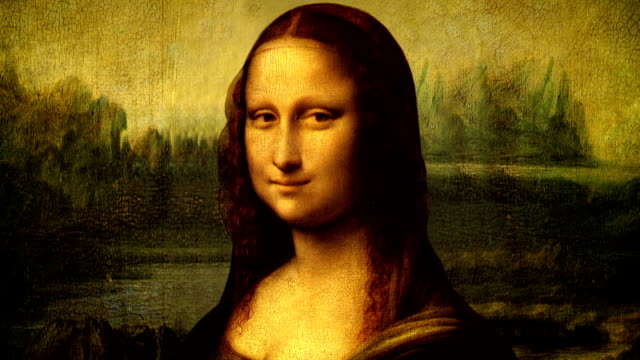
\includegraphics[width = 9cm]{portrait}}; 
    % if necessary the picture may be moved by changing the at (coordinates)
    % width defines the 'zoom' of the picture
\end{tikzpicture}
\hfill\vline\hfill
\end{minipage}
\begin{minipage}[c]{0.4\textwidth}
    \textbf{\Huge \scshape{Charles Rambo}} \\ \vspace{1pt} 
    % \scshape sets small capital letters, remove if desired
    \small{+1 123-456-7890} \\
    \href{mailto:you@provider.com}{\underline{you@provider.com}}\\
    % Be sure to use a professional *personal* email address
    \href{https://www.linkedin.com/in/charles-rambo/}{\underline{linkedin.com/in/charles-rambo}} \\
    % you should adjust you linked in profile name to be professional and recognizable
    \href{https://github.com/fizixmastr}{\underline{github.com/fizixmastr}}
\end{minipage}

% Without picture
%\begin{center}
%    \textbf{\Huge \scshape Charles Rambo} \\ \vspace{1pt} %\scshape sets small capital letters, remove if desired
%    \small +1 123-456-7890 $|$ 
%    \href{mailto:you@provider.com}{\underline{you@provider.com}} $|$\\
%    % Be sure to use a professional *personal* email address
%    \href{https://linkedin.com/in/your-name-here}{\underline{linkedin.com/in/charles-rambo}} $|$
%    % you should adjust you linked in profile name to be professional and recognizable
%    \href{https://github.com/fizixmastr}{\underline{github.com/fizixmastr}}
%\end{center}



\begin{comment}
This CV was written for specifically for positions I was applying for in
academia, and then modified to be a template.

A standard CV is about two pages long where as a resume in the US is one page.
sections can be added and removed here with this in mind. In my experience, 
education, and applicable work experience and skills are the most import things
to include on a resume. For a CV the Europass CV suggests the categories: Work
Experience, Education and Training, Language Skills, Digital Skills,
Communication and Interpersonal Skills, Conferences and Seminars, Creative Works
Driver's License, Hobbies and Interests, Honors and Awards, Management and
Leadership Skills, Networks and Memberships, Organizational Skills, Projects,
Publications, Recommendations, Social and Political Activities, Volunteering.

Your goal is to convey a who, what , when, where, why for every item you share. 
The who is obviously you, but I believe the rest should be done in that order.
For example below. An employer cares most about the degree held and typically 
less about the institution or where it is located (This is still good 
information though). Whatever order you choose be consistent throughout.
\end{comment}

%-----EDUCATION----------------------------------------------------------------
\section{Education}
  \CVSubHeadingListStart
%    \CVSubheading % Example
%      {Degree Achieved}{Years of Study}
%      {Institution of Study}{Where it is located}
    \CVSubheading
      {{Doctor of Philosophy $|$ \emph{\small{Geographic Information Science}}}}{Sep 2014 -- Feb 2019}
      {University College London}{London, UK}
    \CVSubheading
      {{Master of Science $|$ \emph{\small{Geographic Information Systems and Cartography}}}}{Sep 2011 -- July 2014}
      {Peking University}{Beijing, China}
    \CVSubheading
      {{Bachelor of Science $|$ \emph{\small{Chemistry}}}}{Sep 2007 -- July 2011}
      {Peking University}{Beijing, China} 
  \CVSubHeadingListEnd

%-----WORK EXPERIENCE----------------------------------------------------------
\begin{comment}
try to briefly explain what you did and why it is relevant to the position you
are seeking
\end{comment}

\section{Work Experience}
  \CVSubHeadingListStart
%    \CVSubheading %Example
%      {What you did}{When you worked there}
%      {Who you worked for}{Where they are located}
%      \CVItemListStart
%        \CVItem{Why it is important to this employer}
%      \CVItemListEnd
    \CVSubheading
      {Lecturer in Spatial Data Science}{Feb 2019 -- Present}
      {Centre for Advanced Spatial Analysis, UCL}{London, UK}
      \CVItemListStart
        \CVItem{Lecture in postgraduate modules and supervise MSc and PhD projects}        
        \CVItem{Deputy Department Tutor (since 2020)}
      \CVItemListEnd
    \CVSubheading
      {Guest Lecturer}{Jan 2019 -- Present}
      {School of Architecture and Cities, University of Westminster}{London, UK}
      \CVItemListStart
        \CVItem{Lecture in GIS and spatial analysis}
    \CVItemListEnd
    \CVSubheading
      {Teaching assistant}{Oct 2014 -- Jan 2019}
      {Department of Civil, Environmental and Geomatic Engineering}{London, UK}
      \CVItemListStart
        \CVItem{Lectured in “Agent-Based Simulation” as part of the Msc Course Spatio-Temporal Data Mining}
        \CVItem{Led tutorials in R/Python/NetLogo}
      \CVItemListEnd
     \CVSubheading
      {Research assistant}{Oct 2015 -- Jan 2019}
      {Department of Civil, Environmental and Geomatic Engineering}{London, UK}
      \CVItemListStart
        \CVItem{Part of the EPSRC-funded project 'Crime, Policing and Citizenship'}
        \CVItem{Developed algorithms for predicting spatio-temporal crime hot-spots and dashboards}
      \CVItemListEnd
  \CVSubHeadingListEnd

%-----Publications----------------------------------------------------------
\section{Publications}

\vspace{2mm}
\noindent \textbf{\textit{\ \ Most closely related}}
\begin{bibunit}
% \nocite{apsrev42Control}
\nocite{PirieNatPhys2020,MattPRB2020,WebbPRX2019,GozarNanoLett2017,HuangPRL2015}
\putbib[publications]
\end{bibunit}

\vspace{2mm}
\noindent \textbf{\textit{\ \ Other significant publications}}
\newbibstartnumber{6}
\begin{bibunit}
\nocite{apsrev42Control}
\nocite{CominScience2014,ZeljkovicNanoLetters2014,SoumyanarayananPNAS2013,ZeljkovicScience2012,HoffmanScience2002qpi}
\putbib[publications]
\end{bibunit}

%-----PROJECTS AND RESEARCH----------------------------------------------------
\begin{comment}
Ideally the title of the work should speak for what it is. However if you feel
like you should explain more about why the project is applicable to this job,
use item list as is shown in the work experience section.
\end{comment}

\section{Projects and Research}
  \CVSubHeadingListStart
%    \CVSubheading
%      {Title of Work}{When it was done}
%      {Institution you worked with}{unused}
    \CVSubheading
      {{Surface Plasmon Propagation in the Kretschmann-Raether Configuration} $|$ \emph{\small{Python}}}{Fall 2020}
      {University of Eastern Finland}{}
    \CVSubheading
      {{Simulation of Vector Beams Through High Numerical Aperture Lens} $|$ \emph{\small{Python}}}{Fall 2020}
      {University of Eastern Finland}{}
    \CVSubheading
      {Characterization of the Flame-S Spectrometer for Spectral Imaging Research}{Spring 2020}
      {University of Eastern Finland}{}
    \CVSubheading
      {{Free Form Lens Systems for 3D Printing} $|$ \emph{\small{MATLAB, OpTaliX}}}{Spring 2019}
      {University of Eastern Finland}{}
    \CVSubheading
      {Procedures for Plating and Wet-Etching in III-V Semiconductor Devices}{Summer 2019}
      {Finisar Corp.}{}
    \CVSubheading
      {Photo-Filter Characterization for Photometric Identification of Be Stars}{Fall 2017}
      {Austin College}{}
    \CVSubheading
      {Improved Calibrating Equations for Volumetric Soil Moisture Measurement}{Spring 2017}
      {Austin College}{}
    \CVSubheading
      {{Product Design, and Manufacturing Using 3D Printing} $|$ \emph{\small{Autodesk 123D}}}{Fall 2016}
      {Austin College}{}
  \CVSubHeadingListEnd

%-----Publications--------------------------------------------
\begin{comment}
Again the title should have already been enough, but if it is necessary to add
descriptions maintain the consistency from prior sections
Subsections include 'Refereed journals', 'Book chapters', 'Papers under review'
Numbered list
\end{comment}

\section{Publications}
  \CVSubHeadingListStart
%    \CVSubheading % Example
%      {Work Presented}{When}
%      {Occasion}{}
    \CVSubheading
      {Photometric Filter Fidelity and Use for Be Star Identification}{November 2017}
      {Austin College Physics Research Seminar}{}
    \CVSubheading
      {Reflectometry for Volumetric Soil Moisture Measurement}{May 2017}
      {Austin College Atmospheric Physics Fair}{}
    \CVSubheading
      {Design and Manufacturing of Products using 3D Printing}{April 2017}
      {Austin College Student Scholarship Conference}{}
  \CVSubHeadingListEnd


%-----CONFERENCES AND PRESENTATIONS--------------------------------------------
\begin{comment}
Again the title should have already been enough, but if it is necessary to add
descriptions maintain the consistency from prior sections
\end{comment}

\section{Conferences and Presentations}
  \CVSubHeadingListStart
%    \CVSubheading % Example
%      {Work Presented}{When}
%      {Occasion}{}
    \CVSubheading
      {Photometric Filter Fidelity and Use for Be Star Identification}{November 2017}
      {Austin College Physics Research Seminar}{}
    \CVSubheading
      {Reflectometry for Volumetric Soil Moisture Measurement}{May 2017}
      {Austin College Atmospheric Physics Fair}{}
    \CVSubheading
      {Design and Manufacturing of Products using 3D Printing}{April 2017}
      {Austin College Student Scholarship Conference}{}
  \CVSubHeadingListEnd

%-----HONORS AND AWARDS--------------------------------------------------------
\section{Honors and Awards}
  \CVSubHeadingListStart
%    \CVSubheading %Example
%      {What}{When}
%      {Short Description}{}
    \CVSubheading
      {Dean's List}{Fall 2017}
      {Recognition for to 20\% of students in academics at Austin College}{}
    \CVSubheading
      {Noyce STEM Education Leadership Scholarship}{June 2017}
      {Merit based grant for students pursuing education in STEM fields}{}
    \CVSubheading
      {Stephens Scholarship}{May 2017}
      {Merit based scholarship to support international study experiences within Austin College}{}
    \CVSubheading
      {John D . Mosely Scholarship}{July 2016}
      {Merit based scholarship requiring Austin College alumnus nomination}{}
    \CVSubheading
      {Presidents List}{Spring 2016}
      {Overall GPA above 3.8 at Austin College}{}
    \CVSubheading
      {Eagle Scout}{April 2006}
      {Highest level of achievement within the Boy Scouts of America}{}
  \CVSubHeadingListEnd

%-----TEACHING EXPERIENCE------------------------------------------------------
\begin{comment}
Section is here as it applied to my application for positions in academia. 
Remember to tailor the resume for to the position.
\end{comment}

\section{Teaching Experience}
  \CVSubHeadingListStart
%    \CVSubheading
%      {What}{When}
%      {School}{Where}
    \CVSubheading
      {High School Physics (11 Weeks Teaching/Observing)}{Fall 2017}
      {Denison High School}{Denison, TX}
    \CVSubheading
      {High School Calculus (11 Weeks Teaching/Observing)}{Fall 2017}
      {Denison High School}{Denison, TX}
    \CVSubheading
      {High School Geometry (9 Weeks Teaching/Observing)}{Spring 2016}
      {Sherman High School}{Sherman, TX}
  \CVSubHeadingListEnd

%-----COMMUNITY INVOLVEMENT----------------------------------------------------
\section{Community Involvement}
  \CVSubHeadingListStart
%    \CVSubheading %Example
%      {What you did}{When you worked there}
%      {Who you worked for}{Where they are located}
    \CVSubheading
      {Austin College Community Tutors}{Fall 2017 -- Fall 2018}
      {Free tutoring for local students in science and mathematics}{Sherman, TX}
    \CVSubheading
      {River Legacy Nature Center}{September 2015 -- August 2016}
      {Provided assistance for various youth science education programs}{Arlington, TX}
    \CVSubheading
      {Back on My Feet Run Club}{April 2014 -- August 2015}
      {Helping to reestablish homeless persons in the community}{Austin, TX}
  \CVSubHeadingListEnd

%-----SKILLS-------------------------------------------------------------------
\begin{comment}
This section is compressed from the various skills sections that Euro CV
recommends.
\end{comment}

\section{Skills}
 \begin{itemize}[leftmargin=0.5cm, label={}]
    \small{\item{
     \textbf{Languages}{: English (Native), Spanish (B1), Finnish (A1)} \\
     \textbf{Programming}{: Python (NumPy, SciPy, Matplotlib, Pandas), MATLAB, Mathematica, Java} \\
     \textbf{Document Creation}{: Microsoft Office Suite, LaTex, Markdown} \\
    }}
 \end{itemize}
    
%------------------------------------------------------------------------------
\end{document}